\documentclass[12pt]{article}
\setlength\parindent{0pt}
\usepackage{fullpage}
\usepackage{amsmath}
\usepackage{graphicx}
\setlength{\parskip}{4mm}
\def\LL{\left\langle}   % left angle bracket
\def\RR{\right\rangle}  % right angle bracket
\def\LP{\left(}         % left parenthesis
\def\RP{\right)}        % right parenthesis
\def\LB{\left\{}        % left curly bracket
\def\RB{\right\}}       % right curly bracket
\def\PAR#1#2{ {{\partial #1}\over{\partial #2}} }
\def\PARTWO#1#2{ {{\partial^2 #1}\over{\partial #2}^2} }
\def\PARTWOMIX#1#2#3{ {{\partial^2 #1}\over{\partial #2 \partial #3}} }
\newcommand{\BE}{\begin{displaymath}}
\newcommand{\EE}{\end{displaymath}}
\newcommand{\BNE}{\begin{equation}}
\newcommand{\ENE}{\end{equation}}
\newcommand{\BEA}{\begin{eqnarray}}
\newcommand{\EEA}{\nonumber\end{eqnarray}}
\newcommand{\EL}{\nonumber\\}
\newcommand{\la}[1]{\label{#1}}
\newcommand{\ie}{{\em i.e.\ }}
\newcommand{\eg}{{\em e.\,g.\ }}
\newcommand{\cf}{cf.\ }
\newcommand{\etc}{etc.\ }
\newcommand{\Tr}{{\rm tr}}
\newcommand{\etal}{{\it et al.}}
\newcommand{\OL}[1]{\overline{#1}\ } % overline
\newcommand{\OLL}[1]{\overline{\overline{#1}}\ } % double overline
\newcommand{\OON}{\frac{1}{N}} % "one over N"
\newcommand{\OOX}[1]{\frac{1}{#1}} % "one over X"



\begin{document}
\Large
\centerline{\sc{Homework 5}}
\normalsize
\centerline{\sc{Due at the end of the day of Monday, 29 March}}

\begin{enumerate}

%
%\item A jet airplane is flying at a level course at constant speed; the engines are all running at maximum power. 
%
%\begin{itemize}
%
%\item What is the net force on the airplane?
%
%\item Draw a force diagram of the plane as seen from the side with the plane
%flying to the right. Name all of the forces shown on your diagram. 
%
%\item Airplanes bank (tilt to the side) when they turn. Draw a force diagram of the 
%plane as seen from behind as it turns to the left. 
%
%\item Why do airplanes bank as they turn? Explain this by reference to the force diagram you drew.
%\end{itemize}
\item A heavy ball with mass 10 kg is suspended by a rope of length 4.5 m. It is pulled to one side and released, swinging like
a pendulum; at its lowest point, it reaches a speed of 6 m/s. 

\begin{enumerate}
	\item What is the tension in the rope at that point?
	\item Explain in words (without using mathematics) why the tension in the rope here is greater than the weight of the ball.
\end{enumerate}
%
%\item Astrologers\footnote{{\it Astronomy} is the scientific study of the stars. {\it Astrology} is the practice of fortune-telling and divination based on the apparent motion of stars and planets. They are not the same thing. :)} claim that the positions of the planets can influence events on Earth. In this problem,
%you'll calculate whether this is plausible or not.
%
%\begin{enumerate}
%\item Which planet's gravity do you think would have the greatest effect on Earth? Venus' orbit is closest,
%but Jupiter is largest.
%\item Look up astronomical parameters for Earth and your chosen planet. What is the closest they ever
%are to each other? You may approximate their orbits as circles, and can find all the information you need
%on Wikipedia. Show how you estimate their distance of closest approach.
%\item What acceleration does your chosen planet impart to objects on Earth? Is this acceleration relevant 
%to anything?
%\end{enumerate}
%
%\item
%{
%In this exercise, you will think carefully about the meaning of our constant $g$. 
%
%Recall that scales measure the normal force they exert, and the ``apparent weight'' of an object is the normal force exerted on it by the surface below it.
%
%For this exercise, use the ``standard average value'' of $g$ -- 9.8067 $rm m/\rm s^2$. Later we will see why this is not quite a standard -- nor an average.
%
%In this problem, treat the Earth as a sphere with radius 6378 km. This is not quite right (the radius near the equator is a little larger), but it is close enough.
%
%\begin{enumerate}
%
%\item Suppose that Tux the Penguin, with a mass of one kilogram, stands on a scale at the Sorth Pole. What value will the scale read?
%\item Suppose Tux then travels to the Equator and stands on a scale there. What is its {\it acceleration?} (Remember that the Earth is rotating around its axis at an angular velocity of one rotation per day. You will need to convert this to radians per second.)
%\item What is Tux's apparent weight at the Equator?
%\item {This difference suggests that there are two different ways we could define $g$:
%\begin{enumerate}
%	\item ... based on the {\it force of gravity} that an object experiences
%	\item ... or based on the {\it apparent weight} that an object experiences
%\end{enumerate}
%   Which definition do you think is most useful to engineers, and why?
%}
%
%\end{enumerate}
%
%}





%\begin{minipage}{0.7\textwidth}
%\item Two wires are tied to the sphere of mass 3 kg shown here. The sphere
%revolves around the pole in a horizontal circle at constant speed. {\it (Hint: Usually 
%high school geometry isn't that helpful, but here it is. You will need to be a bit clever to
%find the radius of the circle that the ball travels in. As a hint, consider that the triangle formed 
%between the pole and the two wires is isosceles.)}
%
%  \end{minipage}
%  \begin{minipage}{0.3\textwidth}
%\centerline{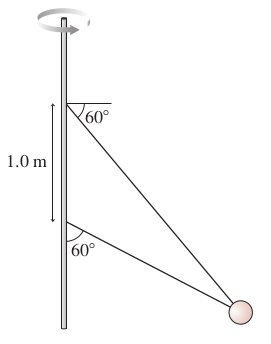
\includegraphics[width=0.9\textwidth]{problem837.png}}
%  \end{minipage}
%
%\begin{enumerate}
%\item For what speed is the tension the same in both wires?
%\item What is that tension?
%\end{enumerate}

\item A ball is attached to the end of a string hanging from the roof of a subway car. 
The train goes around a curve, turning to the left. You know that the car is traveling at 60 km/hr.

\begin{enumerate}
\item Which way will the ball appear to swing?
\item What force pushes the ball in that direction? If there is no such force, explain why the ball swings to the side even though there is no force pushing on it.
\item If the ball swings at an angle of $15^\circ$, what is the radius of curvature of the curve in the tracks?
\end{enumerate}

\begin{minipage}[t]{0.6\textwidth}
\item 

A carnival ride consists of a vertical wheel of radius $r$ rotating at angular velocity $\omega$ around a
horizontal axis. There is a horizontal platform attached to it; a person stands on the platform. (This platform
stays horizontal, and does not rotate; the person remains upright during the whole ride.) This
person has mass $m$, and stands on a scale. The coefficient of static friction between their feet and the scale is 
$\mu_s = 0.5$.
\end{minipage}
\begin{minipage}{0.35\textwidth}
\vspace{0.8in}
\begin{center}
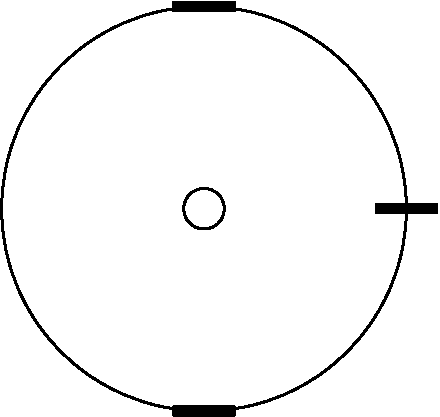
\includegraphics[width=0.8\textwidth]{wheel-crop.pdf}
\end{center}
\end{minipage}

\begin{enumerate}
\item Draw force diagrams for the person at the top of the circle, the bottom of the circle, and the position at the 
same height as the middle of the circle. (You will need to think carefully about the third one of these.)
\item How does the scale reading relate to the forces that act on the person standing on the platform?
\item In terms of $m$, $g$, $r$, $\mu_s$, and $\omega$, what is the scale reading at the top? (Your answer may not depend on all of these.)
\item In terms of $m$, $g$, $r$, $\mu_s$, and $\omega$, what is the scale reading at the bottom? (Your answer may not depend on all of these.)
\item What coefficient of static friction is required for the person not to slide at the position at the same height as the middle, in terms of $m$, $g$, $r$, and $\omega$?
%\item {\bf Extra credit:} If the angular velocity $\omega$ is gradually increased, eventually the person will slide off of the platform. At what location
%will the person slide off? (Hint: It's not any of the three positions marked.)
\end{enumerate}

\item The film {\it Apollo 13} tells the story of three astronauts trying to survive aboard a crippled spacecraft in
space between the Earth and the Moon. It involves scenes where the actors appear to be ``weightless'', mimicking 
the experience of the astronauts. Since going to space was prohibitively expensive, the producers shot those scenes
in a set inside an aircraft. The aircraft flew in parabolas with an acceleration of precisely $g$ downward; during this time,
the astronauts appeared to float inside the set, as the aircraft climbed and then dove toward the ground.

\begin{enumerate}
\item The astronauts were able to experience ``weightlessness'' for about 25 seconds at a time. How far did the aircraft have
to climb and then dive in order to do this?
\item Consider three forms of ``weightlessness'':
\begin{itemize}
\item The experience of the actors and crew of the film {\it Apollo 13} in this aircraft
\item The experience of astronauts in the Space Station, in orbit around Earth at a low altitude
\item The experience of the astronauts in a real deep space mission like {\it Apollo 13}, in which the astronauts flew
400,000 km from Earth (which has a radius of around 6000 km). 
\end{itemize}
What are the similarities between the dynamics of ``weightlessness'' in these situations? What are the differences? 

\end{enumerate}
%
%\item We discussed ``cherry-picking'' in class as an example of misleading science. This is the practice of considering
%only a carefully-chosen subset of data or doing only a limited set of experiments 
%in considering whether a scientific explanation or model agrees with observations
%(usually choosing observations that support the model), rather than including {\it all} available data and 
%conducting experiments that are designed to possibly refute the proposal.
%
%Think of an example in the modern era (since 1875, more or less) where ``cherry-picked'' data have resulted in 
%incorrect scientific claims. (It doesn't matter whether these claims were made by scientists themselves, or by
%other people like politiicans or businessfolk, etc.)  
%
%In a brief discussion of around 250 words, describe the situation, answering questions like:
%
%\begin{itemize}
%\item What happened? What incorrect claims were made, and how were they supported by incomplete data?
%\item Were the people making these claims acting maliciously (intentionally using cherry-picked data to make claims they 
%knew were untrue), or was their use of limited data a result of an honest mistake?
%\item If you were reading their claims at the time, could you have recognized them as 
%misleading?
%\end{itemize}

\end{enumerate}



\end{document}
